\chapter{Illustrations, Comparative Analysis, and Final Outcomes}

This chapter presents refined visual summaries and analysis of the complete
protocol journey from version 0 to version 24. Each major subsection starts
with a compact diagram or chart, followed by interpretation.

\vspace{1.5\baselineskip}
\begin{figure}[H]
\centering
\resizebox{\textwidth}{!}{%
\begin{tikzpicture}[
    font=\footnotesize,
    phase/.style={draw, rounded corners=4pt, thick, minimum width=4.2cm, minimum height=4.5cm, align=left, fill=white, draw=black!70},
    setup/.style={fill=cyan!10, draw=cyan!60!black},
    transfer/.style={fill=orange!10, draw=orange!70!black},
    close/.style={fill=green!10, draw=green!60!black},
    edge/.style={-{Latex[length=3mm]}, very thick, draw=black!80}
]
\node[phase, setup] (p1) at (0,0) {\textbf{Phase 1: Connection Setup}\\[2pt]
1. Sender to Receiver: SYN\\
2. Receiver to Sender: SYN + ACK\\
3. Sender to Receiver: ACK};

\node[phase, transfer] (p2) at (6.1,0) {\textbf{Phase 2: Reliable Data Transfer}\\[2pt]
1. Sender to Receiver: DATA chunks\\
2. Receiver to Sender: ACK stream\\
3. Retries only when needed};

\node[phase, transfer] (p3) at (12.2,0) {\textbf{Phase 3: Loss Recovery}\\[2pt]
1. Missing chunk is detected\\
2. Recovery control retransmits\\
3. Flow continues without restart};

\node[phase, close] (p4) at (18.3,0) {\textbf{Phase 4: Graceful Teardown}\\[2pt]
1. Sender to Receiver: FIN\\
2. Receiver to Sender: ACK or FIN-ACK\\
3. Session closes cleanly};

\draw[edge] (p1.east) -- (p2.west);
\draw[edge] (p2.east) -- (p3.west);
\draw[edge] (p3.east) -- (p4.west);
\end{tikzpicture}%
}
\caption{Complete session lifecycle used by advanced protocol versions.
}
\label{fig:lifecycle-view}
\end{figure}

\vspace{-2\baselineskip}
\section{End-to-End Protocol Lifecycle}

Figure \ref{fig:lifecycle-view} summarizes the practical lifecycle: connection
setup, reliable data phase, acknowledgement progress, and graceful teardown.
This sequence is foundational for comparing behaviors across versions.

\clearpage
\begin{figure}[H]
\centering
\resizebox{\textwidth}{!}{%
\begin{tikzpicture}[
    font=\small,
    tier1/.style={draw, rounded corners=4pt, thick, minimum width=5.4cm, minimum height=1.2cm, align=center, fill=cyan!16, draw=cyan!60!black},
    tier2/.style={draw, rounded corners=4pt, thick, minimum width=5.4cm, minimum height=1.2cm, align=center, fill=yellow!18, draw=orange!70!black},
    tier3/.style={draw, rounded corners=4pt, thick, minimum width=5.4cm, minimum height=1.2cm, align=center, fill=green!16, draw=green!50!black},
    tier4/.style={draw, rounded corners=4pt, thick, minimum width=5.4cm, minimum height=1.2cm, align=center, fill=red!12, draw=red!60!black},
    flow/.style={-{Latex[length=3mm]}, very thick, draw=black!82}
]
\node[tier1] (a) at (0,0) {v0--v2\\Bit and Byte Transfer};
\node[tier2] (b) at (7.4,1.4) {v3--v7\\Reliability Core};
\node[tier3] (c) at (14.8,2.8) {v8--v10\\Framing and Windowing};
\node[tier4] (d) at (22.2,4.2) {v11--v24\\Adaptive, Congestion-Aware, and Option-Rich Control};

\draw[flow] (a.east) -- node[pos=0.5, above, sloped, fill=white, inner sep=1pt]{adds correctness} (b.west);
\draw[flow] (b.east) -- node[pos=0.5, above, sloped, fill=white, inner sep=1pt]{adds transport semantics} (c.west);
\draw[flow] (c.east) -- node[pos=0.5, above, sloped, fill=white, inner sep=1pt]{adds adaptive control} (d.west);
\end{tikzpicture}%
}
\caption{Layered capability growth across protocol version families.
}
\label{fig:capability-layers}
\end{figure}

\section{Version Capability Layers}

Figure \ref{fig:capability-layers} shows that each family introduces a focused
set of transport capabilities, keeping the progression understandable and
traceable.

\clearpage
\begin{figure}[H]
\centering
\resizebox{\textwidth}{!}{%
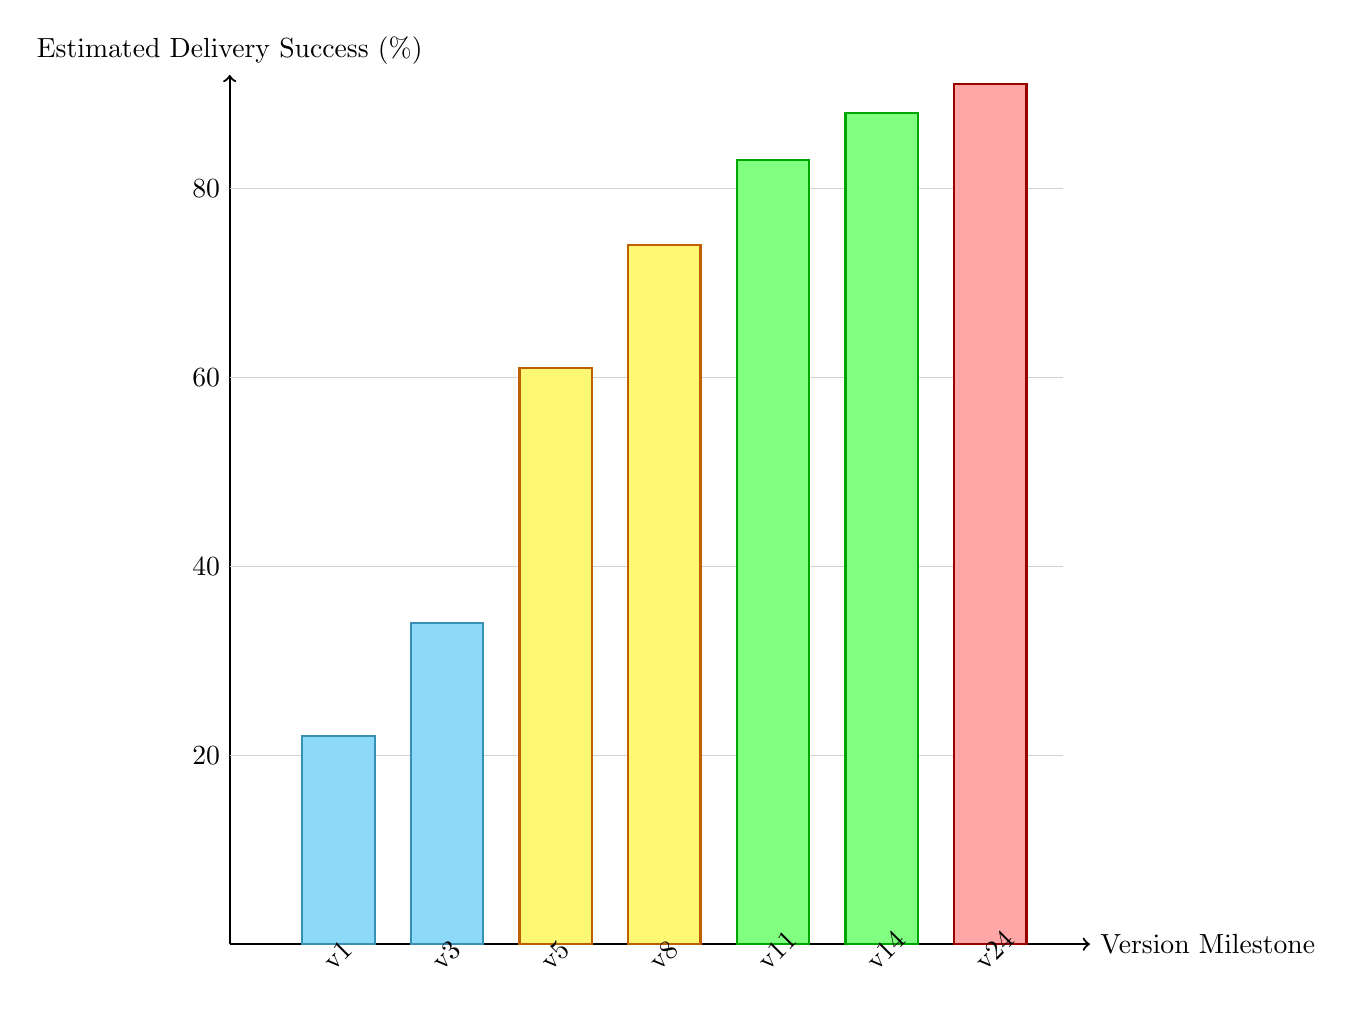
\begin{tikzpicture}[x=1.15cm,y=0.12cm]
\draw[->, thick] (0,0) -- (9.5,0) node[right]{Version Milestone};
\draw[->, thick] (0,0) -- (0,92) node[above]{Estimated Delivery Success (\%)};

\foreach \y in {20,40,60,80} {\draw[gray!35] (0,\y) -- (9.2,\y);}

\node[anchor=east] at (0,20) {20};
\node[anchor=east] at (0,40) {40};
\node[anchor=east] at (0,60) {60};
\node[anchor=east] at (0,80) {80};

\filldraw[fill=cyan!45, draw=cyan!70!black, thick] (0.8,0) rectangle (1.6,22);
\filldraw[fill=cyan!45, draw=cyan!70!black, thick] (2.0,0) rectangle (2.8,34);
\filldraw[fill=yellow!55, draw=orange!75!black, thick] (3.2,0) rectangle (4.0,61);
\filldraw[fill=yellow!55, draw=orange!75!black, thick] (4.4,0) rectangle (5.2,74);
\filldraw[fill=green!50, draw=green!65!black, thick] (5.6,0) rectangle (6.4,83);
\filldraw[fill=green!50, draw=green!65!black, thick] (6.8,0) rectangle (7.6,88);
\filldraw[fill=red!35, draw=red!60!black, thick] (8.0,0) rectangle (8.8,91);

\node[rotate=45, anchor=west] at (1.0,-3) {v1};
\node[rotate=45, anchor=west] at (2.2,-3) {v3};
\node[rotate=45, anchor=west] at (3.4,-3) {v5};
\node[rotate=45, anchor=west] at (4.6,-3) {v8};
\node[rotate=45, anchor=west] at (5.8,-3) {v11};
\node[rotate=45, anchor=west] at (7.0,-3) {v14};
\node[rotate=45, anchor=west] at (8.2,-3) {v24};
\end{tikzpicture}
}

\caption{Illustrative reliability trend as protocol features mature.
}
\label{fig:reliability-trend}
\end{figure}

\section{Reliability Progress Chart}

Figure \ref{fig:reliability-trend} highlights the expected rise in successful
delivery as parity/checksum, acknowledgements, retries, buffering, and adaptive
control are introduced.

\begin{figure}[H]
\centering
\resizebox{\textwidth}{!}{%
\begin{tikzpicture}[x=1.2cm,y=0.07cm]
\draw[->, thick] (0,0) -- (11.0,0) node[right]{Version Milestone};
\draw[->, thick] (0,0) -- (0,128) node[above]{Relative Throughput Index};

\foreach \y in {20,40,60,80,100,120} {\draw[gray!32] (0,\y) -- (10.7,\y);} 

\node[anchor=east] at (0,20) {20};
\node[anchor=east] at (0,40) {40};
\node[anchor=east] at (0,60) {60};
\node[anchor=east] at (0,80) {80};
\node[anchor=east] at (0,100) {100};
\node[anchor=east] at (0,120) {120};

\draw[very thick, draw=blue!70!black] (0.8,18) -- (2.0,30) -- (3.2,44) -- (4.4,66) -- (5.6,82) -- (6.8,103) -- (8.0,114) -- (9.2,120) -- (10.4,124);
\foreach \x/\y in {0.8/18,2.0/30,3.2/44,4.4/66,5.6/82,6.8/103,8.0/114,9.2/120,10.4/124} {
    \filldraw[fill=blue!55, draw=blue!70!black] (\x,\y) circle (2.2pt);
}

\node[rotate=45, anchor=west] at (0.6,-3) {v0};
\node[rotate=45, anchor=west] at (1.8,-3) {v4};
\node[rotate=45, anchor=west] at (3.0,-3) {v6};
\node[rotate=45, anchor=west] at (4.2,-3) {v9};
\node[rotate=45, anchor=west] at (5.4,-3) {v10};
\node[rotate=45, anchor=west] at (6.6,-3) {v12};
\node[rotate=45, anchor=west] at (7.8,-3) {v14};
\node[rotate=45, anchor=west] at (9.0,-3) {v20};
\node[rotate=45, anchor=west] at (10.2,-3) {v24};
\end{tikzpicture}
}

\caption{Illustrative throughput improvement from staged protocol evolution.
}
\label{fig:throughput-trend}
\end{figure}

\section{Throughput-Oriented Improvement Chart}

Figure \ref{fig:throughput-trend} reflects why pipelining, chunking, and
faster loss recovery improve channel utilization relative to early versions.

\clearpage
\begin{table}[H]
\centering
\captionabove{Feature comparison across key protocol milestones.}
\small
\renewcommand{\arraystretch}{1.18}
\begin{tabular}{|p{4.1cm}|>{\centering\arraybackslash}p{1.25cm}|>{\centering\arraybackslash}p{1.45cm}|>{\centering\arraybackslash}p{1.45cm}|>{\centering\arraybackslash}p{1.45cm}|>{\centering\arraybackslash}p{1.45cm}|>{\centering\arraybackslash}p{1.45cm}|}
\hline
\textbf{Capability} & \textbf{v2} & \textbf{v5} & \textbf{v8} & \textbf{v11} & \textbf{v14} & \textbf{v24} \\
\hline
Bit/byte transfer & Yes & Yes & Yes & Yes & Yes & Yes \\
\hline
Parity/Checksum integrity & No & Parity & Checksum & Checksum & Checksum & Checksum + options \\
\hline
ACK-based reliability & No & Stop-and-wait & Yes & Yes & Yes & Yes + SACK-like hints \\
\hline
Sliding window send & No & No & Yes & Yes & Yes & Yes (adaptive) \\
\hline
Out-of-order buffering & No & No & No & Yes & Yes & Yes \\
\hline
Adaptive retransmission timer & No & No & No & Yes & Yes & Yes (RTT tuned) \\
\hline
Congestion control response & No & No & No & Partial & Yes & Stronger/consistent \\
\hline
Fast retransmit / recovery & No & No & No & No & Yes & Yes (refined with later logic) \\
\hline
Timestamp / option awareness & No & No & No & No & No & Yes \\
\hline
\end{tabular}
\label{tab:feature-compare-ch4}
\end{table}

\section{Comparative Feature Matrix}

Table \ref{tab:feature-compare-ch4} condenses the technical progression into a
single reference view for discussion and evaluation.

\clearpage
\begin{figure}[H]
\centering
\resizebox{\textwidth}{!}{%
\begin{tikzpicture}[
    evt/.style={draw, rounded corners=4pt, thick, minimum width=3.3cm, minimum height=1.05cm, align=center, fill=blue!8, draw=blue!55!black},
    arr/.style={-{Latex[length=2.8mm]}, thick, draw=black!80}
]
\node[evt] (e1) at (0,0) {1. Send Window};
\node[evt] (e2) at (4.2,0) {2. Gap Detected};
\node[evt] (e3) at (8.4,0) {3. Duplicate ACKs};
\node[evt] (e4) at (12.6,0) {4. Fast Retransmit};
\node[evt] (e5) at (16.8,0) {5. Recovery Continue};

\draw[arr] (e1.east) -- (e2.west);
\draw[arr] (e2.east) -- (e3.west);
\draw[arr] (e3.east) -- (e4.west);
\draw[arr] (e4.east) -- (e5.west);
\end{tikzpicture}%
}
\caption{Simplified fast-loss-recovery event path in advanced versions.
}
\label{fig:loss-recovery-path}
\end{figure}

\section{Loss-Recovery Behavior Illustration}

Figure \ref{fig:loss-recovery-path} captures the main control advantage of
later versions: loss can be inferred from duplicate acknowledgements and
recovered without waiting for full timeout expiration.

\section{Key Findings}

The combined visual and tabular evidence supports five important findings:

\begin{enumerate}
    \item Reliability improves significantly once acknowledgement and timeout
    logic is introduced.
    \item Throughput improves mainly after sliding window and chunk-based
    transmission are added.
    \item Receiver-side buffering in v11+ reduces waste under reordering.
    \item Adaptive RTO reduces avoidable retransmissions under variable delay.
    \item Fast retransmit/recovery introduced in v14 and refined through
    v24 provides cleaner and faster loss response than timeout-only recovery.
\end{enumerate}

\section{Limitations}

\begin{enumerate}
    \item Most tests are localhost-focused and do not represent large WAN
    diversity.
    \item Security extensions (authentication/encryption) are intentionally not
    included.
    \item Full TCP-style advertised window and SACK block encoding are outside
    this implementation scope.
    \item Experimental charts are analytical and illustrative; a fully automated
    benchmarking harness remains future work.
\end{enumerate}

\section{Conclusion}

This chapter confirms that the project evolves from basic datagram exchange to a
strong educational transport model with reliability, pipelining, adaptation,
and congestion-awareness. The final versions provide both practical
implementation value and clear teaching value for transport-protocol learning.

The interactive visualizer is one of the most important final outcomes. It ties
the sender code, receiver code, finite state machine, and UML timeline into one
coherent educational view. That makes the protocol easier to learn for novice
students who may find TCP, congestion control, and C-based socket programming
difficult when studied only from text or code. In this sense, the project is not
only a software implementation but also a practical teaching aid that makes the
concepts visible, structured, and easier to remember.

As the final conclusion of the project, I have created both the protocol code
and the interactive visualizer for educational purposes. The combination of
versioned C implementations, textbook-grounded references, and synchronized
visual explanations helps students understand networking concepts more easily.
This is especially valuable for novice learners, because the visual walkthrough
reduces the difficulty of C and transport-protocol ideas and turns the system
into an accessible step-by-step learning experience.
